\documentclass{mall}
\usepackage{tikz}
\usepackage{graphicx}
\newcommand{\version}{Version 1.1}
\author{Christer Vesterlund, \url{chrve180@student.liu.se}\\
  Denis I. Blazevic \url{denbl369@student.liu.se}}
\title{Assignment 4:\\Distance Vector Routing}
\date{2017-03-03}
\rhead{Christer Vesterlund\\Denis I. Blazevic}

\begin{document}
\projectpage
\tableofcontents
\newpage 

\section{Task} 
This assignment has two parts. The first part consists of four tasks: design, implementation, test and demonstration of a program in Java that implements a distributed and asynchronous distance vector routing protocol, based on the Bellman-Ford equation. The solution should include the "Poisoned Reverse" technique, which solves the problem of looping in routing topologies
\subsection{Distance vector routing}
Distance-vector routing protocols are one of the two major protocols used. The other one is called link-state protocol, but are not covered in this assignment. We are going to focus on the Bellman-Ford algorithm and in short terms try to explain how this algorithm works.\\

\setlength{\parindent}{0mm}
The basic idea is that each node periodically sends its own distance vector estimate to neighbors When a node x receives new vector estimate from its neighbor, then it updates its own vector using Bellman-Ford equation. A very simple way of describe this kind of routing is to think of it as a graph with a number of nodes. In this graph every node knows its neighbor and the cost to each of them. But this is not enough, because in order to be able to determine the best (minimum cost) to our destination, we need our neighbors minimum cost sent to us when their costs changes. We now have two important pieces of the puzzle:
\begin{enumerate}
\item The direction which the packets should travel to reach its destination.
\item The estimated minimum cost to the destination.
\end{enumerate}
To calculate this cost we use the following equation:
\begin{verbatim}
dx(y) = min v {c(x,v) + d v (y)}
in other words:
dx(y) = cost of least-cost path from X to Y
\end{verbatim}
This is done for all the neighbors to node x. If we find that a cost is lower then the one in our table, our table of costs is updated and so are the routing table. This information is then sent to all neighbors to inform them of our change of costs. When they receive this information, they recalculate theirs cost table.

\subsection{Test of algorithm}
To test our solution we have used the provided graphs. The tests was performed with change of link-costs and without the change of link-costs, to ensure that everything worked as predicted.
\newpage
\subsection{Poison reverse}
If we have a graph with tree nodes with a routing table as follow:
\begin{table}[htb]
\centering
\begin{tabular}{llll}
Node & R1 & R2 & R3\\\hline
R1&     0&	1&	2\\\hline
R2&	1&	0&	1\\\hline
R3&	2&	1&      0\\\hline

\end{tabular}
\end{table}\\
And suddenly the connection between R2 and R3 is lost. Then after one iteration of sending the information, we will get the following routing table:
\begin{table}[htb]
\centering
\begin{tabular}{llll}
Node & R1 & R2 & R3\\\hline
R1&     0&	1&	2\\\hline
R2&	1&	0&	3\\\hline
R3&	2&	3&      0\\\hline

\end{tabular}
\end{table}\\
This happens because R2,R3 is no longer connected, so R2 ``thinks'' it can redirect packages to R3 through R1, which has a path of 2 - so it will get a path of weight 3. And after another iteration, R1 now finds that R2 is more expensive then it used to be and make changes according to this changes.\\

\begin{table}[htb]
\centering
\begin{tabular}{llll}
Node & R1 & R2 & R3\\\hline
R1&     0&	1&	4\\\hline
R2&	1&	0&	3\\\hline
R3&	4&	3&      0\\\hline

\end{tabular}
\end{table}

This will continue until they come to halt at the correct value. The problem here is if R1 or R3 have a high value, then this will become very expensive. This problem is called the ``count to infinity'' problem.\\

One way to handle this kind of problem is to use the technique called ``poison reverse''. The basic idea is that the routing through a node  that has a neighbor node that wants a packet sent to them, lies to the node about the cost between previous node and the next node. This makes the nodes not jump back to the previous node thus eliminating the ``count to infinity'' problem. As a result of this, the packets takes another route. The poisoned node updates its routing table and sends an update back to the node from which it received the route poisoning, to ensure that all nodes gets this update/information.
\pagebreak
\subsubsection{When does Poison Reverse fail?}
Imagine a network with four nodes just like the embedded picture. If node D breaks, then node C will send an update to nodes A and B. Imagine that node B gets the update first, which makes it believe that the best route to node D is through node A. Node C then thinks D is reachable through node B and tells that to node A, thus creating an infinite loop.

\begin{figure}[h]
	\centering
	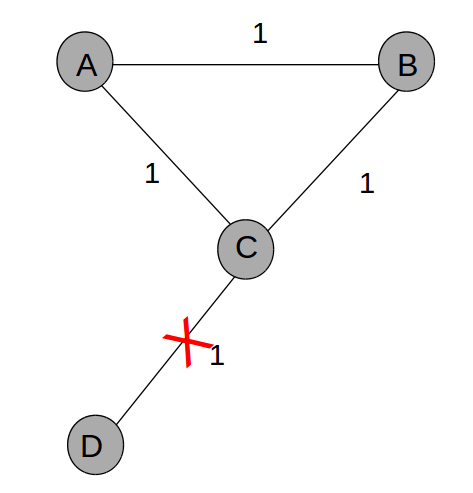
\includegraphics[scale=0.5]{a-b-c-d.png}
\end{figure}

There is three ways of handling routes. These two are the ones used in the lab.
\begin{enumerate}
	\item By using plain ``Bellman-Ford'' algorithm nodes A and B will not have any way to get rid of the loop started by node B's update. 
	\item By using ``Poison Reverse'' nodes A and B will announce an infinite count for the route to each other, which will get rid of the routing loop problem as soon as an update is successfully transmitted.
\end{enumerate}
The third way is better and an solution to the routing problem, even though ``Poison Reverse'' will work with loops with max size of 2 nodes.
\begin{enumerate}
	\setcounter{enumi}{2}
	\item By using the technique ``Split Horizon'' nodes A and B will immediately stop updating and broadcasting the routes to each other, what will happen is that the nodes gets rid of the loops as soon as an route times out. 
\end{enumerate}

\end{document}
 
